\documentclass[11pt]{article}
\usepackage[T1]{fontenc}
\usepackage{lmodern}
\usepackage[margin=1.1in]{geometry}
\usepackage{amsmath,amssymb,amsthm,mathtools,mathrsfs}
\usepackage{microtype}
\usepackage{enumitem}
\usepackage{tikz}
\usepackage{float}
\usetikzlibrary{arrows.meta,calc,positioning}
\usepackage[hidelinks,pdfauthor={OpenAI},pdftitle={A finitely generated counterexample to the Eilenberg--Ganea conjecture}]{hyperref}
\usepackage{bookmark}
\input{glyphtounicode}
\pdfglyphtounicode{arrowhookleft}{21AA}
\pdfglyphtounicode{mapsto}{007C}
\pdfglyphtounicode{parenleftbig}{0028}
\pdfglyphtounicode{parenrightbig}{0029}
\pdfglyphtounicode{vextendsingle}{007C}
\pdfglyphtounicode{vextenddouble}{2225}
\pdfglyphtounicode{parenleftbigg}{0028}
\pdfglyphtounicode{parenrightbigg}{0029}
\pdfglyphtounicode{parenleftBigg}{0028}
\pdfglyphtounicode{parenrightBigg}{0029}
\pdfglyphtounicode{summationtext}{2211}
\pdfglyphtounicode{summationdisplay}{2211}
\pdfglyphtounicode{productdisplay}{220F}
\pdfglyphtounicode{tildewide}{0303}
\pdfgentounicode=1

\let\EGoriginalhookrightarrow\hookrightarrow
\renewcommand{\hookrightarrow}{\mathrel{%
  \pdfliteral direct{/Span << /ActualText <FEFF21AA> >> BDC}%
  \EGoriginalhookrightarrow
  \pdfliteral direct{EMC}}}
\let\EGoriginallongmapsto\longmapsto
\renewcommand{\longmapsto}{\mathrel{%
  \pdfliteral direct{/Span << /ActualText <FEFF27FC> >> BDC}%
  \EGoriginallongmapsto
  \pdfliteral direct{EMC}}}

\AddToHook{env/thebibliography/begin}{\phantomsection\addcontentsline{toc}{section}{References}}
\numberwithin{equation}{section}
\newtheorem{theorem}{Theorem}[section]
\newtheorem{lemma}[theorem]{Lemma}
\newtheorem{proposition}[theorem]{Proposition}
\newtheorem{corollary}[theorem]{Corollary}
\theoremstyle{definition}
\newtheorem{definition}[theorem]{Definition}
\theoremstyle{remark}
\newtheorem{remark}[theorem]{Remark}
\newcommand{\Z}{\mathbb Z}
\newcommand{\Q}{\mathbb Q}
\newcommand{\R}{\mathbb R}
\newcommand{\C}{\mathbb C}
\newcommand{\SU}{\operatorname{SU}}
\newcommand{\cdim}{\operatorname{cd}_{\Z}}
\newcommand{\gdim}{\operatorname{gd}}
\newcommand{\one}{\mathbf 1}
\newcommand{\norm}[1]{\left\lVert#1\right\rVert}
\newcommand{\abs}[1]{\left\lvert#1\right\rvert}
\setlist{topsep=5pt,itemsep=3pt}
\title{A finitely generated counterexample to the\protect\\ Eilenberg--Ganea conjecture}
\author{OpenAI}
\date{September 23, 2026}
\begin{document}
\maketitle
\begin{abstract}
We construct a finitely generated residually finite group of integral cohomological dimension two and geometric dimension three, disproving the Eilenberg--Ganea conjecture.
\end{abstract}
\section{Introduction}
\label{sec:introduction}

For a discrete group $\Gamma$, its integral cohomological dimension $\cdim\Gamma$ is the projective dimension of the trivial left $\Z[\Gamma]$-module $\Z$: it measures the length of the shortest projective resolution of $\Z$. Its geometric dimension $\gdim\Gamma$ is the least dimension of a connected CW complex with fundamental group $\Gamma$ and contractible universal cover. Such a complex is a \emph{classifying space}, or a $K(\Gamma,1)$. These are ordinary dimensions; no family of subgroups or proper-action variant is involved. The cellular chains of a contractible universal cover give a free resolution, so $\cdim\Gamma\le\gdim\Gamma$.

The Eilenberg--Ganea theorem of 1957 identifies these dimensions when $\cdim\Gamma\ge3$. In dimension one, Stallings proved that a finitely generated group of integral cohomological dimension one is free, and Swan removed the finite-generation hypothesis \cite{Stallings1968,Swan1969}; a free group has a one-dimensional classifying space. The remaining dimension-two conjecture asks whether every group of integral cohomological dimension two has a two-dimensional classifying space \cite{EG1957}. We answer this question negatively with a finitely generated residually finite group. Here \emph{residually finite} means that every nonidentity element remains nonidentity in some finite quotient.

Our group comes from a finite simplicial complex. A simplicial complex is \emph{flag} if every finite set of pairwise adjacent vertices spans a simplex. For such a complex $L$ with vertex set $V$, the associated \emph{right-angled Artin group} is
\[
 A_L=\left\langle a_q\ (q\in V)\ \middle|\
 [a_q,a_r]=1\text{ if }\{q,r\}\text{ is an edge of }L\right\rangle.
\]
The \emph{height homomorphism} $\lambda:A_L\to\Z$ sends every standard generator $a_q$ to $1$. Its kernel is a Bestvina--Brady group. Acyclicity below always means vanishing reduced integral homology.

\begin{theorem}
\label{thm:main}
There is a finitely generated residually finite group $G$ such that
\[
 \cdim G=2,\qquad \gdim G=3.
\]
One may take $G$ to be the height kernel in the right-angled Artin group associated to a finite acyclic flag triangulation of the presentation complex
\begin{equation}
\label{eq:seed-presentation-intro}
 \langle x,y\mid x^2=y^5,\ x^2=(xy^{-1})^3\rangle.
\end{equation}
No two-dimensional classifying space for this $G$ exists, regardless of the number of its cells.
\end{theorem}

Section~\ref{sec:geometry} constructs the triangulation and proves the stated algebraic and geometric properties of its height kernel. Finite generation also makes $G$ countable, so restricting the conjecture to countable groups does not restore it.

Proposition~\ref{prop:model} also supplies a length-two resolution of the trivial $\Z[G]$-module $\Z$ by finitely generated free $\Z[G]$-modules. A group admitting such a finite-length free resolution is said to be of \emph{type $\mathrm{FL}$}. Consequently, $G$ is of \emph{type $\mathrm{FP}_\infty$}: it admits a projective resolution with finitely generated terms in every degree. Here the length-two free resolution extends to such a projective resolution by taking all higher terms to be zero. The group is not finitely presented: $L$ has nontrivial fundamental group by Lemma~\ref{lem:geometric-seed}, and the Bestvina--Brady finite-presentability criterion applies \cite[Main Theorem, part~(3)]{BB1997}.

\subsection*{History and the obstruction}

Bestvina and Brady used height kernels to distinguish homological from homotopical finiteness conditions \cite[Main Theorem]{BB1997}. Their acyclic two-dimensional examples provide candidates for the dimension-two problem \cite[Example~6.3(3)]{BB1997}. For suitable flag triangulations of a spine of the Poincar\'e homology sphere, they proved that at least one of the Eilenberg--Ganea and Whitehead conjectures fails \cite[Theorem~8.7]{BB1997}. Whitehead's asphericity question asks whether every connected subcomplex of an aspherical two-dimensional CW complex is aspherical \cite{Whitehead1941}; see also \cite[Section~8]{BB1997}. The classical alternative does not itself determine the geometric dimension of a height kernel. Leary and Petrosyan give a recent conditional comparison between Coxeter and Bestvina--Brady candidates for the ordinary problem \cite[Section~5.6, Conjecture~5.20 and Corollary~5.21]{LP2026}.

Dicks and Leary describe height kernels by edge generators and power relators associated to cycles \cite[Theorem~1 and Proposition~2]{DicksLeary1999}. Howie studied related Bestvina--Brady examples through plus constructions and obtained finite-rank free relation modules \cite{Howie1999}. These works provide the construction and relation-module setting for the present paper. The interface needed here is the particular free basis represented by triangular boundary chains; its exact form is displayed below and proved directly in Proposition~\ref{prop:model}.

The obstacle is that a free action on an acyclic two-complex supplies a short free resolution, whereas a classifying space requires a contractible universal cover. An acyclic complex need not be contractible. Proving that one acyclic model is noncontractible therefore leaves open the possibility of a different two-dimensional classifying space. We compare the cycle module of the acyclic model with the presentation arising from \emph{any} hypothetical two-dimensional classifying space. The comparison permits arbitrary sets of generators and relators in that hypothetical model.

\subsection*{The geometric model and the proof interfaces}

For the complex $L$ in Theorem~\ref{thm:main}, form the union of the coordinate subtori in $(S^1)^V$ indexed by the simplices of $L$, using the common basepoint in all other coordinates. This is a cubical model for $A_L$ with a contractible three-dimensional universal cover $E$. Identify its vertices with $A_L$. The height homomorphism extends affinely over its cubes, and
\[
 X=\lambda^{-1}(0)\subset E
\]
is a two-dimensional level complex with vertex set $G$. The group $G=\ker\lambda$ acts freely on $X$ by left translation, with one vertex orbit and finitely many cell orbits. Proposition~\ref{prop:model} proves that $X$ is acyclic and that $G$ is finitely generated and residually finite, with $\cdim G=2$ and $\gdim G\le3$. These are the geometric inputs to the obstruction; their proofs are included in Section~\ref{sec:geometry}.

Here is the exact algebraic information supplied by $X$. Choose the lift based at $1$ of one oriented edge in each $G$-orbit. Its endpoint is the value of the corresponding letter in a finite generating alphabet $S$ for $G$; distinct edge orbits retain distinct letters. Reading the boundaries of representatives of the triangular two-cell orbits gives a finite indexed list $\mathcal D$ of words on $S$. Write parenthesized superscripts for direct sums. For $\Lambda=\Z[G]$, let $\partial_1:\Lambda^{(S)}\to\Lambda$ be the cellular edge boundary and let $[z]$ be the edge chain of a word $z\in\mathcal D$. The canonical map
\[
 \Lambda^{(\mathcal D)}\longrightarrow\ker\partial_1,
 \qquad e_z\longmapsto[z],
\]
is an isomorphism. Thus the specified boundary chains form a free basis, with both spanning and independence. The words in $\mathcal D$ are trivial in $G$, but they need not be a presentation of $G$; this distinction is the reason for the comparison argument.

We use labels in $H=\SU(2)$, identified with the unit quaternions. An edge labeling assigns an element of $H$ to each oriented edge and the inverse element to its reverse. A \emph{path product} multiplies the labels in traversal order; for a closed path we also call this its \emph{holonomy}. A labeling is \emph{flat on the triangles} when every triangular boundary has product $1$. The two main interfaces give incompatible conclusions about these labels:
\begin{enumerate}
\item Theorem~\ref{thm:presentation} shows that a hypothetical two-dimensional $K(G,1)$ would force every sufficiently small labeling, flat on all translates of the words in $\mathcal D$, to have trivial product along every closed path.
\item Proposition~\ref{prop:small-labels} constructs, for every $\epsilon>0$, labels of distance less than $\epsilon$ from $1$ that are flat on every triangle of $X$ and have nontrivial product along some closed path.
\end{enumerate}
Choosing the second labeling below the threshold in the first statement excludes every two-dimensional classifying space. The quotient $E/G$ supplies a three-dimensional one.

\subsection*{How the comparison and transport work}

Boundary chains record signed edge traversals but forget their order, so equal chains need not give equal path products in $H$. Theorem~\ref{thm:presentation} overcomes this loss of information using an actual aspherical presentation. After adding generators with defining relators, we change the relator words so that a finite distinguished list has exactly the boundary chains $[z]$ supplied by $X$; all additional generators represent the identity of $G$ and therefore give loop edges. The word identities in this presentation yield exact translated signed counts. Once the remaining relator equations hold, these counts cancel the linear discrepancy between the distinguished products and the triangular products. Commutators of elements close to $1$ contribute only a quadratic error. The construction works even if the hypothetical presentation has infinitely or uncountably many generators and relators.

This estimate prevents the distinguished products from reaching a fixed positive distance from $1$ while the prescribed edge labels remain sufficiently small. On a finite quotient, each finite collection of the remaining relator equations has independent vectors recording the total exponents of the unknown labels. The word-equation degree method of Gerstenhaber and Rothaus \cite{GR1962}, with related representation-theoretic applications in Fr\o yshov \cite{Froyshov2013}, supplies the starting point for solving these systems. At the coefficient-free starting system, Lemma~\ref{lem:localized-degree} gives nonzero degree on the conjugation-invariant region where the distinguished products are small. The quadratic barrier preserves this degree as the prescribed labels move to their required values.

Residual finiteness allows us to copy any finite collection of prescribed labels to a suitable quotient. Compactness then gives labels on all additional edges of the original graph. Since the original triangular products are exactly $1$, the same quadratic estimate forces the distinguished products to be exactly $1$ as well. All relators of an actual presentation now vanish, so every closed path has trivial product. The original labeling need not descend to any single finite quotient.

The transport construction contradicts this conclusion. Reduced words in $A_L$ give maps from the graph of $X$ to $L$ whose edge and triangle-boundary images are uniformly small, while special long paths map exactly around prescribed loops of $L$. The seed in Equation~\eqref{eq:seed-presentation-intro} supplies a nontrivial representation $\pi_1(L)\to\SU(2)$. Pulling its transport back along these maps gives small edge labels: the small triangle images force trivial triangular products, and an exactly traced loop detected by the representation retains nontrivial holonomy. Section~\ref{sec:transport} constructs the maps and labels explicitly.

\subsection*{Conventions and organization}

We measure distance in $H$ by the quaternion norm $\abs{a-b}$; this metric is bi-invariant. Our traversal-order convention makes the product along a path followed by another path the product of their respective labels in that order. We use
\begin{equation}
\label{eq:quaternion-basic}
 \abs{a_1\cdots a_k-1}\le\sum_{j=1}^k\abs{a_j-1},
 \qquad
 \abs{ab-ba}\le2\abs{a-1}\abs{b-1}.
\end{equation}
The first inequality follows by telescoping; the second follows by expanding
$ab-ba=(a-1)(b-1)-(b-1)(a-1)$.

Group rings act from the left. Generator edges run from $g$ to $gs$, and translating a path by $g$ means left translation. We work in ordinary set theory with choice, including compactness of products indexed by arbitrary sets.

Section~\ref{sec:degree} proves the localized degree statement. Section~\ref{sec:presentation} derives the presentation obstruction, including its arbitrary-cardinality comparison and compactness steps. Section~\ref{sec:geometry} constructs the seed, the group and the acyclic level model, and Section~\ref{sec:transport} constructs the small labels and completes the contradiction. Standard CW topology, covering-space theory, and finite-dimensional degree theory enter with their stated hypotheses at the relevant steps.

\section{Degree on a conjugation-invariant part of a word fiber}
\label{sec:degree}

The comparison argument will need a solution that remains in a specified
part of a word map's identity fiber as its coefficients vary. A global
degree calculation does not locate that solution. When the exponent-sum matrix is nonsingular, we prove nonvanishing
for any conjugation-invariant isolating part that contains the identity.

Write $H=\SU(2)$ as the group of unit quaternions. We orient $H$ once and give $H^m$ the product orientation. A \emph{word map} $f:H^m\to H^m$ has coordinates that are words in its $m$ arguments and their inverses, without coefficients. Its exponent-sum matrix $B=(B_{ij})$ records the total exponent of the $j$th argument in the $i$th word.

We use ordinary mapping degree on an isolating open set. Thus, if $M$ is a closed oriented $n$-manifold, $f:M\to M$ is smooth, and $y\notin f(\partial\mathcal O)$, then $\deg(f,\mathcal O,y)$ counts the part of $f^{-1}(y)$ in $\mathcal O$. It is defined even when $\partial\mathcal O$ is not smooth. For the compact selected fiber $K=f^{-1}(y)\cap\mathcal O$, map the local orientation class in $H_n(\mathcal O,\mathcal O\setminus K;\Z)$ to $H_n(M,M\setminus\{y\};\Z)\cong\Z$. This relative-homology construction gives excision and homotopy invariance while the boundary avoids $y$; when $y$ is regular it gives the signed count of preimages. We use the relative orientation class over a compact subset from \cite[Lemma~3.27(a)]{Hatcher2002}, together with excision. Regular fibers and the signed-degree and homotopy-invariance facts are supplied by \cite[Section~2, Lemmas~1--2; Section~5, Theorems~A--B]{Milnor1965}.

The global degree formula for compact connected Lie groups goes back to Gerstenhaber and Rothaus \cite[Theorem~1]{GR1962}; for $H=\SU(2)$ it gives $\deg f=\det B$. A coefficient-free formulation also appears in \cite[Proposition~2.1]{Froyshov2013}. We need a statement about an individual invariant part of the fiber. The following proof provides that localization directly.

\begin{samepage}
\begin{lemma}[Localized word-map degree]
\label{lem:localized-degree}
Let $m\ge1$, and let $f:H^m\to H^m$ be a word map with $\det B\ne0$. Suppose that $\mathcal O\subset H^m$ is open, invariant under simultaneous conjugation, contains $\one$, and satisfies
\[
 \partial\mathcal O\cap f^{-1}(\one)=\varnothing.
\]
Then $\deg(f,\mathcal O,\one)\ne0$.
\end{lemma}
\end{samepage}

\begin{proof}
Let $J=\{e^{i\theta}:\theta\in\R\}$ be the standard maximal torus. On $J^m$, the map $f$ is the torus homomorphism with matrix $B$. In particular, its fiber over $\one$ consists of $\abs{\det B}$ points, each regular for the torus restriction, each with tangent sign $\operatorname{sign}(\det B)$. Let $b$ be the number of these points in $\mathcal O$. The identity is one of them, so $b\ge1$.

Fix an odd prime $p>b$. Simultaneous conjugation by $e^{2\pi i/p}$ generates a cyclic group $C_p$ acting on $H^m$. Its fixed set is $J^m$, and the action is free off $J^m$: since $p$ is prime, a nontrivial stabilizer is the whole group. The word map is equivariant. We shall perturb it equivariantly, without changing its restriction to $J^m$, until $\one$ is regular. The fixed preimages will each contribute $\operatorname{sign}(\det B)$, while the others will contribute in multiples of $p$.

\smallskip
\noindent\emph{Regularizing the fixed preimages.}
At a torus root $x$, use left-translated exponential coordinates in the source and exponential coordinates at $\one$ in the target. Since $x$ commutes with $J$, the coordinate actions are the same adjoint representation:
\[
 \R^m\oplus\C^m,
 \qquad (u,v)\longmapsto (u,e^{4\pi i/p}v).
\]
Here the real directions are the $i$-directions, and each complex plane is spanned by $j,k$. An equivariant derivative has no mixed blocks, because the normal rotation has no fixed vector. Its normal block $N$ is complex linear: commuting with the nonreal scalar $e^{4\pi i/p}$ is equivalent to commuting with multiplication by $i$. The tangent block is $B$.

Choose mutually disjoint invariant coordinate neighborhoods of all torus roots. Each can be chosen entirely inside $\mathcal O$ or entirely outside its closure, because no root lies on the boundary. In one such chart add
\[
 (u,v)\longmapsto s\chi(u,v)(0,v)
\]
to the coordinate expression of $f$, where $\chi$ is an invariant smooth bump function equal to one near the root. Choose $s\in\R$ arbitrarily small with $\det_{\C}(N+sI)\ne0$; only finitely many real values are excluded. This changes neither the torus restriction nor the tangent block. The resulting derivative is invertible, and its sign is
\[
 \operatorname{sign}(\det B)\,
 \operatorname{sign}\det_{\R}(N+sI)
 =\operatorname{sign}(\det B),
\]
since the real determinant of an invertible complex linear map is positive. The coordinate orientations can be chosen compatibly in source and target. Each fixed preimage is now isolated and regular.

\smallskip
\noindent\emph{Regularizing the remaining preimages.}
Choose an invariant open neighborhood of each regular fixed root, with closure contained in a coordinate neighborhood where that root is the only zero. Keep the map unchanged near the closures of the chosen neighborhoods. The zero set outside their union is closed in $H^m$, hence compact. It lies in the free-action locus: a sequence of these remaining zeros approaching $J^m$ would limit to a torus root, already inside one of the chosen neighborhoods.

Cover this compact set by finitely many smaller coordinate neighborhoods, each inside a larger neighborhood whose $p$ translates are disjoint. Different families of translates need not be disjoint from one another. Choose the closures of the bump supports to map into a smaller target logarithm ball, and keep the parameters small enough that every perturbed value stays in the larger exponential coordinate ball. In these target coordinates, add a vector parameter times a bump function in each larger neighborhood, and propagate the change to its translates by equivariance. Choose the bumps positive on the smaller neighborhoods. Near every remaining zero at least one parameter block therefore gives a surjective derivative to the target. By compactness, sufficiently small perturbations introduce no zeros elsewhere outside the protected fixed-root neighborhoods.

The joint map of source point and parameters is consequently transverse to $\one$ near all its zeros. The regular-value theorem and Sard's theorem, applied to the projection of its zero manifold onto parameter space, give arbitrarily small parameter values for which the slice has only regular zeros. These are standard finite-dimensional results; no equivariant transversality theorem is needed on the fixed set. All perturbations can be kept uniformly small enough that $\partial\mathcal O$ stays disjoint from the fiber over $\one$, since this boundary is compact. Homotopy invariance preserves the selected degree.

Every nonfixed zero of the resulting equivariant map occurs in an orbit of $p$ points. The local signs in an orbit agree: conjugation preserves the orientations of both source and target. The signed-count formula thus gives
\[
 \deg(f,\mathcal O,\one)
 \equiv b\,\operatorname{sign}(\det B)\pmod p.
\]
The right side is nonzero modulo $p$, since $0<b<p$. The degree is therefore nonzero.
\end{proof}

\begin{remark}
The same argument works for arbitrarily large odd primes, so it actually gives
$\deg(f,\mathcal O,\one)=b\,\operatorname{sign}(\det B)$.
Only nonvanishing is needed below. When there are no variables and no equations, the corresponding map is the identity of a point, with degree one.
\end{remark}

\section{Comparison with an arbitrary aspherical presentation}
\label{sec:presentation}

Let $\Gamma$ be a group with a finite generating alphabet $S$.
Distinct letters are kept distinct, even if they have the same value in
$\Gamma$.  Its generator graph has vertices $g\in\Gamma$ and an oriented
edge $(g,s)$ from $g$ to $gs$ for each $s\in S$.
Put $\Lambda=\Z[\Gamma]$, acting on chains on the left.  For a word $w$
on $S$, write $\bar w$ for its value in $\Gamma$ and $[w]$ for the chain
of the path starting at $1$.  Thus
\[
 \partial_1:\Lambda^{(S)}\longrightarrow\Lambda,
 \qquad \partial_1(e_s)=s-1,
 \qquad \partial_1[w]=\bar w-1.
\]
Here and throughout this section, a parenthesized superscript denotes a
\emph{direct sum}.  All words and all chains have finite support.

\begin{theorem}[The presentation comparison theorem]
\label{thm:presentation}
Suppose that $\Gamma$ is residually finite and that $\mathcal D$ is a
finite indexed list of words on $S$, trivial in $\Gamma$, whose chains
form a free $\Lambda$-basis of $\ker\partial_1$.  Thus the canonical map
\begin{equation}\label{eq:cycle-basis}
 \Lambda^{(\mathcal D)}\longrightarrow\ker\partial_1,
 \qquad e_z\longmapsto[z],
\end{equation}
is an isomorphism.
If $\Gamma$ admits a $K(\Gamma,1)$ of dimension at most two, there is an
$\eta>0$ with the following property.  Assign a label in $H=\SU(2)$ to
every oriented generator edge, assign the inverse label to its reverse,
and assume that every label has distance less than $\eta$ from $1$.
If the product along every translate of every $z\in\mathcal D$ is $1$,
then the product along every closed edge path is $1$.
\end{theorem}

The words in $\mathcal D$ need not present $\Gamma$.  This distinction is
the reason a comparison argument is necessary.  We first arrange an
arbitrary aspherical presentation so that its relators include a finite
list with chains exactly $[z]$.  The remaining relators give independent
word equations in additional loop labels.  A uniform quadratic estimate
isolates the small values of the distinguished relators.  We solve finite
systems on finite group quotients by Lemma~\ref{lem:localized-degree},
and then use compactness to obtain an extension of the original labels.
The presentation used in this argument can have any cardinality.

\subsection{A presentation with distinguished boundary chains}

The correspondence between relator operations and group-ring boundary
operations is classical; compare Fox's transformation~(III) in
\cite[Section~2]{Fox1954}. We give the word realization explicitly
because the presentation here may have arbitrary index sets.

\begin{lemma}\label{lem:aligned-presentation}
Under the hypotheses of Theorem~\ref{thm:presentation}, including the
existence of the two-dimensional $K(\Gamma,1)$, there is a presentation
\[
 \Gamma=\langle S,\mathcal T\mid
        (\rho_z)_{z\in\mathcal D},\ (r)_{r\in\mathcal R}\rangle
\]
with the following properties:
\begin{enumerate}
\item every letter of $\mathcal T$ has value $1$ in $\Gamma$;
\item the complete relator boundary list is a $\Lambda$-basis of the
cycle module of the generator graph on $S\amalg\mathcal T$;
\item $[\rho_z]=[z]$ as edge chains, for each $z\in\mathcal D$;
\item projecting the ordinary boundaries $[r]$, $r\in\mathcal R$, to
the $\mathcal T$-edge coordinates gives an isomorphism
\begin{equation}\label{eq:ordinary-projection}
 \Lambda^{(\mathcal R)}\xrightarrow{\ \cong\ }
 \Lambda^{(\mathcal T)}.
\end{equation}
\end{enumerate}
No finiteness assumption is imposed on $\mathcal T$ or $\mathcal R$.
\end{lemma}

\begin{proof}
Start with any two-dimensional $K(\Gamma,1)$.  Collapse a maximal tree
in its connected one-skeleton and replace the two-cell attaching loops
by finite edge words.  These operations preserve the homotopy type:
a contractible CW subcomplex can be collapsed, and homotopic attaching
maps give homotopy equivalent adjunction spaces
\cite[Propositions~0.17 and~0.18]{Hatcher2002}.  These facts apply to
infinite CW complexes as well; a loop in a graph is homotopic to a finite
edge path.  The resulting presentation complex has one vertex, with
some sets of generators and relators.  Its universal cover is acyclic
and has no cells above dimension two.  Consequently its relator boundary
map is an isomorphism onto the cycle module.  The relator words also
normally generate the kernel of the map from the free generator group
to $\Gamma$.

Adjoin the prescribed letters $S$, with one definition relator for each
letter.  Each new relator boundary has coefficient $1$ on its own new
edge and coefficient $0$ on the other new edges.  Subtracting these
boundaries reduces any cycle uniquely to an old cycle, so the boundary
basis property persists.  For each former generator $a$, choose a word
$w_a(S)$ with value $a$ in $\Gamma$, and replace $a$ by $t_a w_a(S)$.
This is an invertible change of free generators: its inverse sends
$t_a$ to $a w_a(S)^{-1}$ and fixes $S$.  The new letters $t_a$ all have
value $1$.  On edge chains the substitution fixes the $S$-edges and
sends $e_a$ to $e_{t_a}+[w_a]$, so it is a chain isomorphism and preserves
the boundary basis property.  Let $T$ be the set of these new letters,
$R$ the current relator index set, and $I=\mathcal D\amalg T$.
Equation~\eqref{eq:cycle-basis} identifies the cycle module with
$\Lambda^{(I)}$.  In these coordinates the relator boundary map is an
isomorphism
\[
 A:\Lambda^{(R)}\longrightarrow\Lambda^{(I)}.
\]

We next arrange that the prescribed cycles themselves occur as relator
boundaries. An auxiliary copy of the cycle module allows the three
shears below to move this basis into a new relator block.
Adjoin letters $U=(u_i)_{i\in I}$ and defining relators $u_i$.
The stabilized boundary map is
\[
 D_0=\begin{pmatrix}A&0\\0&1\end{pmatrix}:
 \Lambda^{(R)}\oplus\Lambda^{(I)}
 \longrightarrow\Lambda^{(I)}\oplus\Lambda^{(I)},
\]
where the second target summand consists of the $U$-edges.  On its
domain put
\[
 P=\begin{pmatrix}1&A^{-1}\\0&1\end{pmatrix},
 \qquad Q=\begin{pmatrix}1&0\\-A&1\end{pmatrix}.
\]
These are blocks of homomorphisms of left modules; all products below
mean composition.  Direct multiplication gives
\begin{equation}\label{eq:presentation-shears}
 PQP=\begin{pmatrix}0&A^{-1}\\-A&0\end{pmatrix},
 \qquad
 D_0PQP=\begin{pmatrix}0&1\\-A&0\end{pmatrix}.
\end{equation}

We realize each of the successive precompositions $P,Q,P$ by actual
relator words.  A shear leaves one block of words unchanged and adds to
each boundary in the other block a finite sum
$\sum_k n_k g_k[b_k]$ of translates of unchanged boundaries.
Choose a generator word $v_k$ representing $g_k$ and multiply the
changing relator by copies of $v_k b_k^{\pm1}v_k^{-1}$, with the indicated
multiplicities and signs.  All these words represent $1$ in $\Gamma$;
the added boundary is precisely the stated sum.  The unchanged words
belong to both old and new relator lists, so the old changing word is
recovered from the new one by a finite inverse multiplication.  Thus
the old and new lists have exactly the same normal closure.
Every column of $A$ and $A^{-1}$ has finite support because their domains
and targets are direct sums.  Hence this construction uses finite words
for every relator even when the index sets are uncountable.  It does
not require an infinite product of words or a limiting sequence of
presentation moves.

In the final second block, the relator indexed by $i\in I$ has boundary
$(e_i,0)$.  Designate those indexed by $z\in\mathcal D$ as $\rho_z$.
Set $\mathcal T=T\amalg U$.  The remaining second-block relators are
indexed by $T$, and the first-block relators are indexed by $R$; these
are the ordinary relators, with $\mathcal R=T\amalg R$.  Their projected
boundary map is, in these orders,
\begin{equation}\label{eq:ordinary-diagonal}
 \begin{pmatrix}1_T&0\\0&-A\end{pmatrix}:
 \Lambda^{(T)}\oplus\Lambda^{(R)}
 \xrightarrow{\ \cong\ }
 \Lambda^{(T)}\oplus\Lambda^{(I)}.
\end{equation}
Equation~\eqref{eq:presentation-shears} also shows that the complete
boundary list remains a basis.  Normal closure was preserved at every
step, so these are the relators of an actual presentation of $\Gamma$.
\end{proof}

The relators now form an actual presentation, and their boundaries are
aligned with the chosen cycle basis. The next step extracts information
that survives evaluation in the nonabelian group $H$: exact signed
counts will cancel the linear error, leaving a quadratic estimate.

\subsection{Exact counts and a uniform quadratic estimate}

Fix the presentation supplied by Lemma~\ref{lem:aligned-presentation}.
For every $z\in\mathcal D$, choose a finite normal-closure expression
in the free group on $S\amalg\mathcal T$:
\begin{equation}\label{eq:relator-expression}
 z=\prod_{j=1}^{n_z}u_{z,j}\,r_{z,j}^{\sigma_{z,j}}u_{z,j}^{-1},
 \qquad \sigma_{z,j}\in\{1,-1\}.
\end{equation}
Each $r_{z,j}$ is an indexed final relator, ordinary or distinguished.
Let $\mathcal T_0\subset\mathcal T$ consist of the finitely many extra letters
appearing in the words $u_{z,j}$.  For each $t\in\mathcal T_0$, also fix a finite
expression of $t$ as a product of conjugates of final relators and their
inverses.  Finally choose a finite set $\mathcal A\subset\mathcal R$
containing every ordinary relator used in these expressions, both
those for $z$ and those for $t$.

\begin{lemma}\label{lem:exact-counts}
In the free module on all final relator indices,
\begin{equation}\label{eq:translated-counts}
 \sum_{j=1}^{n_z}\sigma_{z,j}\bar u_{z,j}e_{r_{z,j}}
       =e_{\rho_z}.
\end{equation}
\end{lemma}
\begin{proof}
The boundary of a conjugate $u r^{\sigma}u^{-1}$ is
$\sigma\bar u[r]$: the two conjugating paths cancel as chains because
$r$ has group value $1$.  Every factor in
Equation~\eqref{eq:relator-expression} also has value $1$, so multiplying
the factors introduces no further prefix translations in its chain.
Applying the complete relator boundary isomorphism to the left side of
Equation~\eqref{eq:translated-counts} therefore gives $[z]$.
The right side has the same image, namely $[\rho_z]=[z]$.
Injectivity gives the asserted equality, coefficient by coefficient.
\end{proof}

We will use labels either on $\Gamma$ or on any finite quotient $F$ of
$\Gamma$.  In the latter case the graph is formed with the prescribed
images of the generators, retaining distinct edges for distinct alphabet
letters even when their images coincide.  All extra-generator edges are loops in
either graph.  Write $L(w,v)$ for the product of the labels along the
word $w$ starting at $v$, in traversal order.  Endpoints depend only on
the group values of the letters, not on their labels.  Consequently
free word identities can be evaluated on these graphs.  In particular,
\[
 L(u r^{\sigma}u^{-1},v)
   =L(u,v)L(r,v\bar u)^{\sigma}L(u,v)^{-1}
 \quad\text{if }\bar r=1,
\]
with group values projected to $F$ when appropriate.

\begin{lemma}[Uniform estimate]\label{lem:quadratic-estimate}
There is a constant $C\ge1$, depending only on the finite choices above,
with the following property on $\Gamma$ and on every finite quotient.
Suppose that all $S$-labels have distance at most $\epsilon$ from $1$,
and that all translates of the ordinary relators in $\mathcal A$
have product $1$.  Put
\[
 h=\sup_{z\in\mathcal D,\ v}|L(\rho_z,v)-1|,
\]
where the supremum is $0$ if $\mathcal D$ is empty.  If
$0\le h,\epsilon\le1$, then, for every $z\in\mathcal D$ and vertex $v$,
\begin{align}
 |L(z,v)-L(\rho_z,v)|&\le C(h+\epsilon)h,
                      \label{eq:quadratic-estimate}\\
 |L(z,v)-1|&\le C\epsilon.\label{eq:short-word-estimate}
\end{align}
\end{lemma}

\begin{proof}
For unit quaternions, telescoping products and bi-invariance give
\begin{equation}\label{eq:quaternion-estimates}
 \left|\prod_{j=1}^n a_j-\prod_{j=1}^n b_j\right|
       \le\sum_{j=1}^n|a_j-b_j|,
 \qquad
 |ab-ba|\le2|a-1|\,|b-1|.
\end{equation}
The second inequality follows by expanding
$ab-ba=(a-1)(b-1)-(b-1)(a-1)$.
Inverses and conjugation preserve distance from $1$.

Evaluate the fixed expression for each $t\in\mathcal T_0$ at any vertex.
Ordinary relators disappear, and every distinguished factor has
distance at most $h$ from $1$, regardless of its conjugator.  Thus
\[
 |L(t,v)-1|\le M h\qquad(t\in\mathcal T_0)
\]
for one finite constant $M$, independent of the vertex and the group
quotient.  No bound on the conjugators in these auxiliary expressions
is required.  Each $u_{z,j}$ uses only letters of $S\amalg\mathcal T_0$, so another
fixed constant $K$ gives
\[
 |L(u_{z,j},v)-1|\le K(\epsilon+h).
\]
On evaluating Equation~\eqref{eq:relator-expression}, discard its
ordinary factors.  Removing the conjugation from a remaining factor
costs at most
\[
 |aba^{-1}-b|=|ab-ba|
       \le 2K(\epsilon+h)h,
\]
including when the relator occurs with exponent $-1$.
There are at most $n_z$ such factors.

The resulting factors are values of distinguished relators, or their
inverses, at specified vertices.  Any interchange of two adjacent
factors costs at most $2h^2$, by
Equation~\eqref{eq:quaternion-estimates}.  Group together occurrences
having the same relator index and the same vertex; at most
$n_z(n_z-1)/2$ interchanges are needed.  Their signed multiplicities
are prescribed exactly by Equation~\eqref{eq:translated-counts},
translated from $1$ to $v$.  On a finite quotient, coincident vertices
merely add the corresponding coefficients, so the same identity
still applies.  After cancellation within each group, the product is
exactly $L(\rho_z,v)$.  The total error is bounded by
\[
 2n_zK(\epsilon+h)h+n_z(n_z-1)h^2.
\]
Since $\mathcal D$ is finite, this proves
Equation~\eqref{eq:quadratic-estimate} with one $C$.
The word $z$ contains only $S$-letters, so
$|L(z,v)-1|\le\operatorname{length}(z)\epsilon$.
Increasing $C$ proves Equation~\eqref{eq:short-word-estimate} as well.
If the distinguished list is empty, the two assertions are vacuous
and any $C\ge1$ suffices.
\end{proof}

Fix from now on numbers $0<\delta<1$ and $0<\eta<1$ such that
\begin{equation}\label{eq:small-thresholds}
 C(\delta+\eta)<\tfrac12,
 \qquad C\eta<\tfrac{\delta}{2}.
\end{equation}
Under the hypotheses of Lemma~\ref{lem:quadratic-estimate}, with
$\epsilon\le\eta$, the value $h=\delta$ is impossible.  Indeed, taking
the supremum in its two inequalities gives
\begin{equation}\label{eq:no-threshold-crossing}
 \begin{aligned}
 h&\le C\epsilon+C(h+\epsilon)h;\\
 h=\delta&\ \Longrightarrow\
 \delta\le C\eta+C(\delta+\eta)\delta<\delta.
 \end{aligned}
\end{equation}
The supremum need not be attained for this argument.

The constants $C$, $\delta$, and $\eta$ are now fixed, independently of
any finite quotient or finite collection of equations. The exclusion of
$h=\delta$ will keep the degree calculation inside the region of small
distinguished products while the prescribed labels move.

\subsection{Solving finite systems by degree}

\begin{lemma}\label{lem:finite-quotient-solvability}
Let $F$ be any finite quotient of $\Gamma$, and prescribe arbitrary
$S$-edge labels on $F$ of distance less than $\eta$ from $1$.
For every finite set $\mathcal B\subset\mathcal R$ containing
$\mathcal A$, there are labels on all $\mathcal T$-edges such that
\[
 L(r,v)=1\quad(r\in\mathcal B,\ v\in F),
 \qquad
 \max_{z\in\mathcal D,\ v\in F}|L(\rho_z,v)-1|<\delta.
\]
The maximum over an empty distinguished list is interpreted as $0$.
\end{lemma}

\begin{proof}
Tensor the isomorphism~\eqref{eq:ordinary-projection} with the right
$\Lambda$-module $\Z[F]$.  This gives an isomorphism
\begin{equation}\label{eq:quotient-basis}
 \Z[F]^{(\mathcal R)}\xrightarrow{\ \cong\ }
 \Z[F]^{(\mathcal T)}.
\end{equation}
No flatness claim is involved: tensoring the inverse gives an inverse
to the displayed map.  As an abelian-group basis, the source has indices
$(v,r)\in F\times\mathcal R$.  Its image consists of the projected
boundary chains of $r$ based at $v$.  Thus the chains for
$F\times\mathcal B$ are linearly independent over $\Q$.

Give an unknown $x_{v,t}\in H$ to each extra edge $(v,t)$.
In the equation $L(r,v)=1$, the exponent count of each unknown is
exactly its coefficient in the projected boundary chain.  This holds
even though the fixed $S$-labels need not commute: the path traversed
is determined by the generator values in $F$, and all $t\in\mathcal T$
have value $1$.  Write the $m=|F|\,|\mathcal B|$ exponent vectors as
rows.  Their union of supports is finite, and their row rank is $m$.
Choose $m$ unknowns giving a nonsingular $m\times m$ integer minor
$B$, and set every other extra label equal to $1$.

Move all the prescribed $S$-labels from $1$ to their final values
along the short quaternion arcs, with common parameter $\tau\in[0,1]$.
These arcs stay at distance less than $\eta$ from $1$.
The selected equations now define a continuous family of smooth maps
\[
 f_\tau:H^m\longrightarrow H^m.
\]
For an assignment $x\in H^m$, let
\[
 h(\tau,x)=\max_{z\in\mathcal D,\ v\in F}
       |L_\tau(\rho_z,v;x)-1|,
 \qquad \mathcal O_\tau=\{x:h(\tau,x)<\delta\}.
\]
Only finitely many words occur here, so $h$ is continuous.
Every root $f_\tau(x)=\one$ satisfies all equations from $\mathcal A$.
Equation~\eqref{eq:no-threshold-crossing} therefore implies
\begin{equation}\label{eq:root-isolation}
 f_\tau(x)=\one\quad\Longrightarrow\quad h(\tau,x)\ne\delta.
\end{equation}
If $m=0$, the domain and target are points.  The unique assignment
starts with $h=0$, and continuity together with
Equation~\eqref{eq:root-isolation} keeps $h<\delta$ throughout.
This proves the assertion in that case; henceforth assume $m\ge1$.

We justify degree invariance with these moving open sets.  For fixed
$\tau_0$, the roots with $h(\tau_0,x)<\delta$ form a compact set:
by~\eqref{eq:root-isolation} they are also the roots with
$h(\tau_0,x)\le\delta$.  Choose an open neighborhood $V$ containing
exactly these roots, with
$\overline V\subset\mathcal O_{\tau_0}$.
If there are no such roots, take $V=\varnothing$.
Compactness of $H^m$ and continuity show that, for all $\tau$ sufficiently
close to $\tau_0$, every root with $h(\tau,x)<\delta$ lies in $V$,
every root in $\overline V$ has $h(\tau,x)<\delta$, and there is no
root on $\partial V$.  For example, a sequence of selected roots
outside $V$ with parameters tending to $\tau_0$ would have a limit
root with $h\le\delta$, hence $h<\delta$, outside $V$, a contradiction.
The other assertions follow in the same way, or from
$\overline V\subset\mathcal O_{\tau_0}$.
Excision and homotopy invariance of ordinary degree now give
\[
 \deg(f_\tau,\mathcal O_\tau,\one)
       =\deg(f_\tau,V,\one)
       =\deg(f_{\tau_0},V,\one)
\]
near $\tau_0$.  Thus the selected degree is locally constant, and hence
constant on $[0,1]$.

At $\tau=0$, the map $f_0$ is a pure word map with exponent matrix $B$:
all fixed coefficients are $1$.  The set $\mathcal O_0$ is invariant
under simultaneous conjugation, contains the identity assignment,
and its boundary contains no root.  Lemma~\ref{lem:localized-degree}
therefore gives
\[
 \deg(f_0,\mathcal O_0,\one)\ne0.
\]
The same holds at $\tau=1$, so a root exists in $\mathcal O_1$, as
required.
\end{proof}

Finite quotients now provide solutions for every finite set of ordinary
relators, with the distinguished products uniformly bounded. To return
to the original graph, we must preserve its prescribed $S$-labels exactly.
The following compactness argument does this one finite collection of
constraints at a time.

\subsection{Finite-coordinate compactness and the conclusion}

We use compactness of arbitrary products of compact spaces
\cite[Theorem~37.3]{Munkres2000}. Its unrestricted index set is essential:
the set of extra generators in the hypothetical presentation need not
be countable.

\begin{proof}[Proof of Theorem~\ref{thm:presentation}]
Let $a$ be any prescribed labeling of the $S$-edges on $\Gamma$ satisfying
the theorem's hypotheses, with the fixed $\eta$ of
Equation~\eqref{eq:small-thresholds}.  In the compact product
\[
 \mathscr P=H^{\Gamma\times\mathcal T}
\]
consider all the following conditions on the unknown extra-edge labels:
\begin{align}
 L(r,g)&=1 &&(r\in\mathcal R,\ g\in\Gamma),
                           \label{eq:compact-ordinary}\\
 |L(\rho_z,g)-1|&\le\delta
             &&(z\in\mathcal D,\ g\in\Gamma).
                           \label{eq:compact-distinguished}
\end{align}
Each condition is closed and depends on finitely many coordinates.
We verify the finite intersection property, keeping the original
labeling $a$ fixed throughout.

First choose an arbitrary finite collection $\mathscr C$ of the
conditions~\eqref{eq:compact-ordinary}--\eqref{eq:compact-distinguished}.
Let $P\subset\Gamma$ be the finite set of starting vertices of all
\emph{positively oriented} $S$-edges used when evaluating the words
in $\mathscr C$.  An inverse occurrence traversing the edge from
$g$ to $gs^{-1}$ uses the positively oriented edge starting at
$gs^{-1}$, and this starting vertex is included in $P$.
Let $\mathcal B$ contain $\mathcal A$ and all ordinary relator indices
appearing in $\mathscr C$.  These choices are made before choosing a
finite quotient.

Residual finiteness supplies a finite quotient
$q:\Gamma\twoheadrightarrow F$ that is injective on $P$:
separate the finitely many nonidentity elements $p^{-1}p'$ for distinct
$p,p'\in P$, and let $F$ be the image of $\Gamma$ in the product
of the resulting finite quotients.
For each $S$-edge actually used in $\mathscr C$, assign to its image
edge in $F$ its prescribed label from $a$.  Injectivity on $P$ ensures
that no two inconsistent prescriptions are placed on the same edge.
Give every remaining $S$-edge of $F$ label $1$.  All these labels have
distance less than $\eta$ from $1$.

Apply Lemma~\ref{lem:finite-quotient-solvability} to this finite quotient,
this assignment, and $\mathcal B$.  Pull the resulting extra-edge labels
back by $q$, and combine them with the \emph{original} $S$-labels $a$
on $\Gamma$.  In every word from $\mathscr C$, each traversed $S$-edge
has the same label as its image in $F$, by construction; the same is
true for each extra edge by pullback.  Its path product therefore
agrees with the quotient path product.  The selected ordinary equations
hold, and the selected distinguished products even have distance
strictly less than $\delta$.  This supplies a point of $\mathscr P$
satisfying $\mathscr C$.

We have proved: for each finite collection of constraints, one can
choose a finite quotient, copy the finitely many required prescribed
labels, solve a finite system there, and pull back a solution to that
collection.  The quotient may depend on the collection; the original
assignment $a$ is never assumed to descend to any one finite quotient.
Compactness of $\mathscr P$ now gives an extension satisfying
all of~\eqref{eq:compact-ordinary}--\eqref{eq:compact-distinguished}
simultaneously.

For this extension, $h\le\delta$ and all the equations in $\mathcal A$
hold.  The original hypothesis says $L(z,g)=1$ for every $z$ and $g$.
Taking suprema in Equation~\eqref{eq:quadratic-estimate}, with
$\epsilon=\eta$, gives
\[
 h\le C(h+\eta)h\le C(\delta+\eta)h<\tfrac12h
 \quad\text{if }h>0.
\]
Thus $h=0$.  All distinguished relators, as well as all ordinary
relators, have product $1$ at every vertex.
Finally, a closed edge path spells a word representing $1$ in $\Gamma$.
Because Lemma~\ref{lem:aligned-presentation} gives an actual presentation,
that word is a finite product of conjugates of final relators and their
inverses.  Evaluating at the starting vertex makes every factor $1$.
Hence the original closed path has product $1$, as claimed.
\end{proof}

\section{An acyclic level model for a height kernel}\label{sec:geometry}

We use the height-kernel construction of Bestvina and Brady
\cite{BB1997}.  We give the geometric details, including the integral
acyclicity statements that will supply the boundary basis required in
Section~\ref{sec:presentation}.

\subsection{A finite seed with quaternion monodromy}

\begin{lemma}\label{lem:geometric-seed}
There is a finite, connected, two-dimensional flag simplicial complex
$L$ with $\widetilde H_*(L;\Z)=0$ and a nontrivial homomorphism
$\alpha:\pi_1(L)\longrightarrow H=\SU(2)$.
\end{lemma}

\begin{proof}
Start with the presentation complex $K$ of
\begin{equation}\label{eq:seed-presentation}
 \langle x,y\mid x^2y^{-5},\ x^2(xy^{-1})^{-3}\rangle.
\end{equation}
The presented group also occurs in Hatcher
\cite[Example~2.38]{Hatcher2002}, with relations
$a^5=b^3=(ab)^2$: take $a=y$ and $b=y^{-1}x$.
Indeed, $x^2=y^5$ is central and $b$ is conjugate to $xy^{-1}$.
We verify the acyclicity of $K$ and construct the required
$\SU(2)$ representation directly.

Its cellular boundary $C_2(K;\Z)\to C_1(K;\Z)$ has exponent-sum
rows $(2,-5)$ and $(-1,3)$.  Their determinant is $1$, so this boundary
is an isomorphism.  Since $K$ has one vertex and no cells above
dimension two, it is integrally acyclic.

Identify $H$ with the unit quaternions.  Put $\theta=\pi/5$ and choose
imaginary unit quaternions $u,v$ with
\[
 u\mathbin{\cdot}v=\frac{1}{2\sin\theta};
\]
this is possible because $\sin\theta>1/2$.  Send $x$ to $u$ and $y$ to
$\cos\theta+v\sin\theta$.  Then $x^2$ and $y^5$ both map to $-1$.
Moreover, the real part of $u(\cos\theta-v\sin\theta)$ is $1/2$.
A unit quaternion with real part $1/2$ has cube $-1$, so both relations
in \eqref{eq:seed-presentation} hold.  The homomorphism is nontrivial
because the image of $x$ is $u\ne1$.

Here is a flag triangulation that avoids any assumption that a
presentation complex is regular.  Subdivide each circle of its
one-skeleton into at least three edges.  Express the two attaching
maps as polygonal edge paths, and cone the boundary of each polygon
to a new interior vertex before making the boundary identifications.
Keep the radial edges indexed by the boundary occurrences: distinct
occurrences of the same graph vertex give distinct radial edges.
Every sector is now a closed triangle with three distinct vertices,
and its closure is embedded.  Indeed, its one outer edge is embedded
in the subdivided graph, while its two radial edges have disjoint
interiors.  Thus this is a finite regular CW structure on $K$.

Take the order complex of its nonempty cells, ordered by inclusion of
closures.  This triangulates $K$: inductively triangulate cell
boundaries and cone each such triangulation from an interior point
of the cell.  Regularity makes these constructions compatible on
common faces.  The result is two-dimensional, and it is flag, since
pairwise comparable cells form a chain.  Call it $L$.  The resulting
homeomorphism transfers both acyclicity and the nontrivial
homomorphism to $L$.
\end{proof}

Fix this $L$ and $\alpha$ for the rest of the paper.  Write $V$ for
its finite vertex set and put
\begin{equation}\label{eq:height-kernel}
 \begin{gathered}
 P=A_L=
 \left\langle a_q\ (q\in V)\ \middle|\
 [a_q,a_r]=1\text{ if }\{q,r\}\in L\right\rangle,
 \\
 \lambda:P\longrightarrow\Z,\quad \lambda(a_q)=1,
 \qquad G=\ker\lambda.
 \end{gathered}
\end{equation}
The map $\lambda$ is well defined and surjective.  We shall prove all
the properties of $G$ needed below directly.

\subsection{Residual finiteness and the cubical universal cover}

Residual finiteness is classical for graph products of residually finite
groups \cite[Corollary~5.4]{Green1990}; see also
\cite[Theorem~3.7]{HsuWise1999}. The following induction includes the
retract-separation argument in the form needed here; compare
\cite[Lemma~3.9(1)]{HsuWise1999}.

\begin{lemma}\label{lem:graph-group-rf}
The group associated to any finite commutation graph is residually
finite.  In particular, $P$ and $G$ are residually finite.
\end{lemma}

\begin{proof}
We induct on the number of vertices.  Delete one vertex, with
generator $t$, and let $P'$ be the group on the remaining graph.
The neighbors of the deleted vertex generate the graph group $C$.
Both inclusions into $P'$ and into the original group are injective:
killing the other generators gives retractions.  Let
$r:P'\to C$ be the first of these retractions.  There is an isomorphism
\begin{equation}\label{eq:graph-group-splitting}
 P\cong F(P'/C)\rtimes P',
\end{equation}
where $P'/C$ denotes left cosets, $F(P'/C)$ is the free group on
symbols $b_{qC}$, and $P'$ acts by left translation of their indices.
To verify the formula, map $P'$ identically to the second factor and
$t$ to $b_C$.  This respects the relations $[t,c]=1$ for $c\in C$.
Conversely, send $b_{qC}$ to $qtq^{-1}$.  This is independent of the
representative of $qC$ and respects the semidirect-product action.
The maps are inverse on the indicated generators.

By induction $P'$ is residually finite.  For $g\notin C$, we have
$g\ne r(g)$, so some finite quotient $p$ of $P'$ satisfies
$p(g)\ne p(r(g))$.  The map $(p,p\circ r)$ separates $g$ from $C$:
every element of $C$ has equal coordinates, whereas $g$ does not.
Taking a product of finitely many such maps shows that any finite
list of distinct left cosets in $P'/C$ remains distinct in
$D/\overline C$ for a suitable finite quotient $D$ of $P'$, where
$\overline C$ is the image of $C$.

Consider a nonidentity element $(w,q)$ of
\eqref{eq:graph-group-splitting}.  If $q\ne1$, a finite quotient of
$P'$ separates it from the identity.  If $q=1$, choose $D$ preserving
the distinct indices appearing in the nonempty reduced free word
$w$.  Its image is still nontrivial in
$F(D/\overline C)\rtimes D$.  A free group is residually finite:
for a nonempty reduced word of length $n$, prescribe its successive
steps on distinct points $0,\ldots,n$.  For each free generator these
steps prescribe an injective partial permutation, because the word
has no adjacent inverse letters.  Complete each partial permutation
to a permutation of this finite set.  The resulting finite
permutation representation sends $0$ to $n$ along the word.
Apply this fact to obtain a finite-index normal subgroup $N$ of
$F(D/\overline C)$ not containing the image of $w$.  Intersect the
finitely many translates of $N$ under $D$.  The intersection is
normal, has finite index, is $D$-invariant, and still omits $w$.
Its quotient, semidirect $D$, is the required finite quotient.
This proves the induction.  Residual finiteness passes to subgroups,
so it also holds for $G$.
\end{proof}

We now use the cubical construction in
\cite[Theorem~5.12]{BB1997}, giving a direct proof of its needed
properties. Let $S_L$ be the union, inside the coordinate torus $(S^1)^V$, of
the coordinate subtori corresponding to the simplices of $L$,
including the common basepoint.  Use the usual one-vertex cell
structure on each circle.  This gives $S_L$ a cubical cell structure,
with one $k$-cube for each clique of size $k$.  Its two-skeleton gives
the presentation of $P$ in \eqref{eq:height-kernel}.  Since $L$ is flag
and two-dimensional, $S_L$ has dimension three.  Let $E$ be its
universal cover.  Identify the vertices of $E$ with $P$ so that an
edge in the positive $q$-direction runs from $p$ to $pa_q$; deck
transformations act by multiplication on the left.

\begin{lemma}\label{lem:cubical-cover}
The space $E$ is a locally finite, contractible, three-dimensional
cubical complex.  Its cubes are embedded, and two intersecting cubes
intersect in a common face.
\end{lemma}

\begin{proof}
First we prove acyclicity of the universal cover for every finite
commutation graph, by induction on its number of vertices.  Use
$t,P',C$ as in the preceding proof.  Downstairs, the cubical complex
is obtained from $S_{P'}$ by attaching
$S_C\times[0,1]$, identifying both ends with the coordinate
subcomplex $S_C\subset S_{P'}$.  Here $S_{P'}$ and $S_C$ denote the
same coordinate-torus construction for those graphs.

Upstairs, the components over $S_{P'}$ are its universal covers,
indexed by left cosets $P/P'$, and the lifted cylinders are products
of the universal cover of $S_C$ with $[0,1]$, indexed by $P/C$.
These covering assertions follow from the injectivity of the
subgroup inclusions.  The cylinder indexed by $gC$ joins the vertex
spaces indexed by $gP'$ and $gtP'$.  Its incidence graph is a tree.
Indeed, under \eqref{eq:graph-group-splitting}, write $g=wq$ with
$w\in F(P'/C)$ and $q\in P'$.  The vertex cosets are identified with
$w$, and this cylinder runs from $w$ to $wb_{qC}$.  The incidence
graph is therefore the Cayley tree of the free group $F(P'/C)$.

By induction every vertex space and every cylinder cross-section
is acyclic.  The union over a finite subtree is acyclic: adjoining
a leaf amounts to gluing in its vertex space and incident cylinder
along one acyclic cylinder end, and the assertion follows from
Mayer--Vietoris.  Any cellular cycle in $E$ meets only finitely many
vertex spaces and cylinders, hence lies in such a finite-subtree
union.  It bounds there.  This proves acyclicity of $E$.  The base
case, the empty graph, is a point.

As a universal cover, $E$ is simply connected.  A simply connected
acyclic CW complex is contractible: a first nonzero homotopy group
would, by the Hurewicz theorem, give a nonzero homology group, and
the Whitehead theorem then applies to the map to a point.  These
are the usual CW forms of the two theorems; see
\cite[Sections~4.1--4.2]{Hatcher2002}.

For completeness, consider the cubical structure itself.  A cube
is specified by its initial vertex $p$ and a clique $\sigma$; its
vertices are
\[
 p\prod_{q\in\tau}a_q,\qquad \tau\subseteq\sigma.
\]
They are distinct by the abelianization map
$P\to\Z^V$.  Each lifted face is determined by its initial vertex
and its direction subset; distinct faces of one cube have distinct
such data, again by abelianization.  Thus every closed cube is
embedded.  Suppose two cubes contain a vertex $p$.  Seen from $p$,
each has a set of distinct signed directions $a_q^{\varepsilon_q}$,
with mutually commuting underlying generators.  Abelianization
shows that any common vertex is obtained from $p$ using only the
equally signed directions shared by the two cubes.  These directions
span the same face in each cube, by uniqueness of lifts.  It contains
all common vertices and hence every common cell.  Since the
intersection is a union of common cells, it is exactly this face.
Every nonempty intersection contains such a vertex.  Finally, only
finitely many signed cliques are available at a vertex, proving
local finiteness.  The three-dimensional assertion follows from
the existence of two-simplices in $L$.
\end{proof}

Extend $\lambda$ affinely over every cube of $E$.  On a cube with
initial vertex $p$ and coordinates $x_1,\ldots,x_k\in[0,1]$, it is
\begin{equation}\label{eq:affine-height}
 \lambda(p)+x_1+\cdots+x_k.
\end{equation}
These formulas agree on faces, and
$\lambda(gx)=\lambda(g)+\lambda(x)$.  In particular, $G$ preserves
the level
\begin{equation}\label{eq:zero-level}
 X=\lambda^{-1}(0).
\end{equation}

The ambient complex $E$ is contractible, and its quotient by $G$ already
gives the three-dimensional classifying space. To obtain the required
length-two resolution, we must instead prove that the two-dimensional
level $X$ is acyclic. This is a homological assertion about the level;
we do not assert that the level is contractible.

\subsection{Acyclicity of the level}

\begin{lemma}\label{lem:acyclic-level}
The level $X$ is a connected, integrally acyclic, two-dimensional
simplicial complex.  Its vertices are $G$, its edges are the integer
level diagonals of squares, and its two-simplices are integer level
sections of three-cubes.
\end{lemma}

\begin{proof}
Triangulate each cube of $E$ by chains in its Boolean poset of
vertices: a simplex is a chain under the order of increasing
coordinates.  These triangulations agree on faces.  Heights are
strictly increasing along every such chain; in particular, no edge
of this triangulation joins vertices of equal height.

At a vertex $p$, the full subcomplex of its link spanned by vertices
of height greater than $\lambda(p)$ is the barycentric subdivision
of $L$.  Indeed, a higher vertex adjacent to $p$ in the triangulation
is obtained by multiplying by the positive generators of a nonempty
clique, and a simplex of these vertices corresponds exactly to a
chain of such cliques.  This description remains valid when $p$ is
an intermediate corner of a cube, since any comparable higher corner
changes only positive directions.  We call this the ascending link.
The descending link is described identically using negative
directions, and is also a subdivision of $L$.  Both links are
integrally acyclic.

Let $K_n$ be the full subcomplex of the triangulation spanned by
vertices of height at least $-n$, for $n\ge0$.  To pass from $K_n$ to
$K_{n+1}$, add simultaneously the vertices $p$ of height $-n-1$ and
the cones on their ascending links.  No simplex contains two of
these new vertices.  Consequently the relative cellular chain
complex is the direct sum, over the new vertices, of
\[
 C_*\bigl(\operatorname{cone}(\operatorname{Asc}(p)),
                   \operatorname{Asc}(p);\Z\bigr).
\]
Each summand has zero homology, since its base is acyclic and
nonempty.  Hence $K_n\hookrightarrow K_{n+1}$ induces an isomorphism
on all homology groups.  This argument explicitly allows infinitely
many vertices at each height.  The union of the $K_n$ is $E$, and
cellular chains have finite support, so homology commutes with this
union.  Thus $K_0\hookrightarrow E$ is a homology isomorphism.
Using descending links in the same way, the full subcomplex on
vertices of height at most zero is also acyclic.

The closed halfspace $E_+=\lambda^{-1}([0,\infty))$ deformation
retracts onto $K_0$.  To see this directly, write a point in a
triangulated simplex as $\sum_i t_iv_i$ and discard the weights of
vertices of negative height, renormalizing the others:
\[
 R_+\left(\sum_i t_iv_i\right)
   =\frac{\sum_{\lambda(v_i)\ge0}t_iv_i}
          {\sum_{\lambda(v_i)\ge0}t_i}.
\]
The denominator is positive on $E_+$: otherwise all vertices with
positive weight would have negative height, contrary to the affine
height of the point.  The linear homotopy from the point to $R_+$
stays in the same simplex and in $E_+$.  It fixes $K_0$, and its
formulas agree on faces.  Local finiteness gives a continuous global
homotopy.  The corresponding construction retracts
$E_-=\lambda^{-1}(( -\infty,0])$ onto the full subcomplex on
nonpositive-height vertices.  Thus both closed halfspaces are
acyclic.

Cut the triangulation along height zero, and subdivide the resulting
polytopes if desired.  The spaces $E_+$, $E_-$, and their intersection
$X$ are then subcomplexes, so the reduced Mayer--Vietoris sequence
applies to $E=E_+\cup E_-$.  Since $E$ and the two halfspaces are
acyclic and $X$ contains the vertex $1$, that sequence proves
$\widetilde H_*(X;\Z)=0$, including connectedness.

For the final cell structure on $X$, return to the original cubes.
The integer slices of $[0,1]^2$ by $x_1+x_2=m$ are a vertex or,
for $m=1$, the diagonal joining $(1,0)$ to $(0,1)$.  The nondegenerate
integer slices of $[0,1]^3$ are the triangles at sums $1$ and $2$.
Slices of edges introduce no new vertices.  Formula
\eqref{eq:affine-height} therefore gives exactly the asserted
vertices, edges, and triangles.  The face-intersection property in
Lemma~\ref{lem:cubical-cover} makes them a simplicial complex.
Triangles occur by taking a three-cube whose initial vertex has
height $-1$, so its dimension is two.  Figure~\ref{fig:level-slices}
illustrates the positive-dimensional slices.
\end{proof}

\begin{figure}[H]
\centering
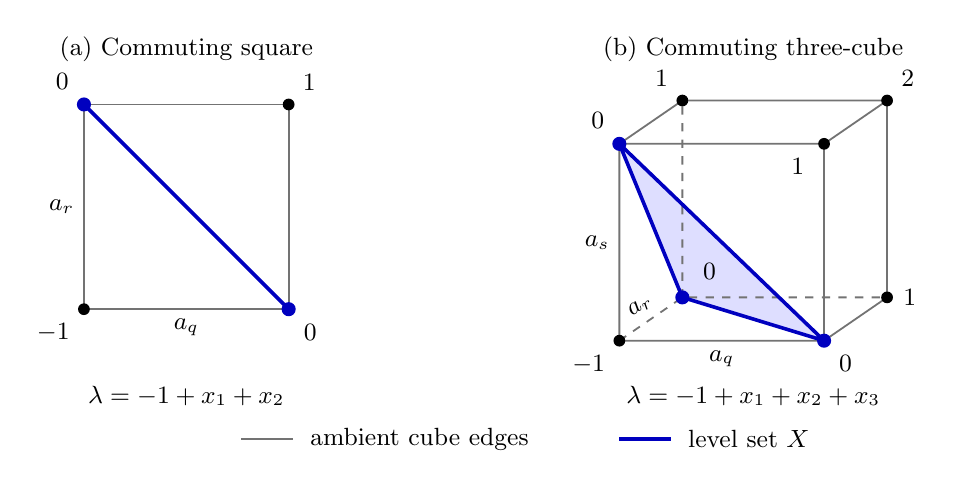
\begin{tikzpicture}[
  font=\small, line join=round,
  ambient/.style={draw=black!55,line width=.65pt},
  level/.style={draw=blue!75!black,line width=1.3pt},
  dot/.style={circle,fill=black,inner sep=1.5pt},
  zero/.style={circle,fill=blue!75!black,inner sep=1.8pt}]
  \begin{scope}[shift={(0,.4)}]
    \coordinate (A) at (0,0);
    \coordinate (B) at (2.6,0);
    \coordinate (C) at (0,2.6);
    \coordinate (D) at (2.6,2.6);
    \draw[ambient] (A)--(B)--(D)--(C)--cycle;
    \draw[level] (B)--(C);
    \node[dot,label=below left:$-1$] at (A) {};
    \node[zero,label=below right:$0$] at (B) {};
    \node[zero,label=above left:$0$] at (C) {};
    \node[dot,label=above right:$1$] at (D) {};
    \node[below] at (1.3,0) {$a_q$};
    \node[left] at (0,1.3) {$a_r$};
  \end{scope}
  \node at (1.3,3.7) {(a) Commuting square};
  \node at (1.3,-.7) {$\lambda=-1+x_1+x_2$};
  \begin{scope}[shift={(6.8,0)}]
    \coordinate (O) at (0,0);
    \coordinate (Q) at (2.6,0);
    \coordinate (R) at (.8,.55);
    \coordinate (S) at (0,2.5);
    \coordinate (QR) at (3.4,.55);
    \coordinate (QS) at (2.6,2.5);
    \coordinate (RS) at (.8,3.05);
    \coordinate (QRS) at (3.4,3.05);
    \fill[blue!13] (Q)--(R)--(S)--cycle;
    \draw[ambient,dashed] (O)--(R)--(QR) (R)--(RS);
    \draw[ambient] (O)--(Q)--(QR)--(QRS)--(RS)--(S)--cycle
      (Q)--(QS)--(S) (QS)--(QRS);
    \draw[level] (Q)--(R)--(S)--cycle;
    \node[dot,label=below left:$-1$] at (O) {};
    \node[zero,label=below right:$0$] at (Q) {};
    \node[zero,label={[xshift=2pt,yshift=1pt]above right:$0$}]
      at (R) {};
    \node[zero,label=above left:$0$] at (S) {};
    \node[dot,label=right:$1$] at (QR) {};
    \node[dot,label={[xshift=-2pt]below left:$1$}] at (QS) {};
    \node[dot,label=above left:$1$] at (RS) {};
    \node[dot,label=above right:$2$] at (QRS) {};
    \node[below] at (1.3,0) {$a_q$};
    \node[left] at (0,1.25) {$a_s$};
    \path (O)--node[above,sloped,pos=.48] {$a_r$} (R);
  \end{scope}
  \node at (8.5,3.7) {(b) Commuting three-cube};
  \node at (8.5,-.7) {$\lambda=-1+x_1+x_2+x_3$};
  \draw[ambient] (2,-1.25)--(2.65,-1.25);
  \node[right] at (2.75,-1.25) {ambient cube edges};
  \draw[level] (6.8,-1.25)--(7.45,-1.25);
  \node[right] at (7.55,-1.25) {level set $X$};
\end{tikzpicture}
\caption{Integer slices of cubes; vertex labels are heights. The blue
diagonal and triangle are an edge and a two-simplex of $X$. Each
generator increases height by one. Initial height $-2$ gives the other
triangular slice, at $x_1+x_2+x_3=2$.}
\label{fig:level-slices}
\end{figure}

The edge and triangular-word descriptions belong to the presentation
framework of Dicks and Leary \cite[Theorem~1 and Proposition~2]{DicksLeary1999}.
We now pass from the level geometry to the precise algebraic input for
Theorem~\ref{thm:presentation}. The finite cell orbits will give finite
alphabets, and acyclicity in both dimensions one and two will give an
isomorphism onto the cycle module, not merely a collection of generators.

\subsection{The group and its boundary basis}

\begin{proposition}\label{prop:model}
The finite flag complex $L$, its nontrivial representation
$\alpha:\pi_1(L)\to H$, and the group $G$ of
\eqref{eq:height-kernel} have the following properties.
\begin{enumerate}
\item $G$ is countable, finitely generated, and residually finite,
      with $\cdim(G)=2$ and $\gdim(G)\le3$.
\item $G$ acts freely on the integrally acyclic two-dimensional
      simplicial complex $X$ of \eqref{eq:zero-level}.  The action
      has finitely many cell orbits and one vertex orbit, identified
      with $G$ acting on itself on the left.
\item There is a finite generating alphabet $S$ for $G$ and a
      finite indexed list $\mathcal D$ of words trivial in $G$ such
      that, for $\Lambda=\Z[G]$, the graph of $X$ has edges
      $g\to gs$ and
      \begin{equation}\label{eq:model-resolution}
       0\longrightarrow\Lambda^{(\mathcal D)}
       \xrightarrow{\ \partial_2\ }\Lambda^{(S)}
       \xrightarrow{\ \partial_1\ }\Lambda
       \xrightarrow{\ \mathrm{aug}\ }\Z\longrightarrow0
      \end{equation}
      is exact, with $\partial_1(e_s)=s-1$ and
      $\partial_2(e_z)=[z]$.  Here $[z]$ is the oriented edge chain
      of the triangular boundary word $z$ based at $1$.
      In particular, the chains $[z]$, $z\in\mathcal D$, are a
      free $\Lambda$-basis of $\ker\partial_1$.
\end{enumerate}
\end{proposition}

\begin{proof}
The first two lemmas supply $L$, $\alpha$, and residual finiteness.
The cubical deck action restricts to $G$ on $X$.  It preserves the
cell structure just described, and no nonidentity element stabilizes
a cell: such an element would preserve its unique ambient open cube
in $E$, hence also that cube's initial vertex.  The action is free,
being the restriction of a deck action.  Vertices of $X$ are exactly
the elements of $G$, so there is one vertex orbit.

There are only finitely many cell orbits.  An ambient cube is
specified by its clique of directions and its initial vertex; a
nonempty integer slice has only finitely many possible relative
heights.  Two initial vertices of the same height differ by left
multiplication by an element of $G$.  Hence the finite list of
cliques and possible relative heights accounts for all the orbits.
The quotient $Y=X/G$ is thus a finite complex with one vertex, and
$X\to Y$ is a regular $G$-cover.  One can obtain this covering by
restricting $E\to E/G$.

Choose orientations for the edge orbits.  For each orbit choose its
oriented lift starting at $1$, and call its endpoint $s\in G$.
Keep different edge orbits as different letters even if their
values coincide; this defines $S$.  Left translation identifies
every oriented edge with $g\to gs$.  Connectedness of $X$ implies
that its graph is connected, so $S$ generates $G$.

For each triangle orbit choose an orientation, a starting corner,
and the lift having that corner at $1$.  Reading its boundary gives
a word $z$ on $S$, necessarily trivial in $G$.  These indexed words
form $\mathcal D$.  The cellular chains of $X$, with the chosen cell
orbit representatives, are precisely the free modules in
\eqref{eq:model-resolution}.  Acyclicity makes the augmented chain
complex exact.  In particular, $H_2(X;\Z)=0$ and the absence of
three-cells make $\partial_2$ injective, which gives the asserted
basis rather than only a spanning set.

This free resolution proves $\cdim(G)\le2$.  To obtain the
opposite inequality, choose a two-simplex of $L$ with vertices
$q,r,s$.  The three corresponding commuting generators form an
embedded $\Z^3$ in $P$: their map from $\Z^3$ is injective after
abelianization in $\Z^V$.  Its height kernel is a subgroup
$\Z^2\subset G$.  Cohomological dimension cannot increase upon
restriction to a subgroup, because a free group-ring module remains
free over the subgroup ring, and consequently projective modules
remain projective.  The torus resolution gives
$H^2(\Z^2;\Z)\cong\Z$, so $\cdim(G)\ge2$.

Finally, $P$ is finitely generated, hence countable, and so is $G$.
The contractible three-dimensional complex $E$ is also a free
$G$-complex; the quotient $E/G$ is a three-dimensional $K(G,1)$.
Thus $\gdim(G)\le3$, completing the proof.
\end{proof}

\section{Small transport with nontrivial holonomy}\label{sec:transport}

Retain the finite flag complex $L$, the homomorphism
$\alpha:\pi_1(L)\to H=\SU(2)$, and the level complex $X$ of
Proposition~\ref{prop:model}.  Write $V$ for the vertex set of $L$ and
$a_v$ for the corresponding standard generator of $P=A_L$.
We realize $|L|$ in $\R^V$ by barycentric coordinates and give it the
metric induced by the $\ell^1$ norm.  Our aim is the following.

\begin{proposition}\label{prop:small-labels}
For every $\epsilon>0$, the oriented edges of $X$ admit labels
$h_e\in H$ such that
\[
 h_{\bar e}=h_e^{-1},\qquad |h_e-1|<\epsilon,
\]
the product around every triangular two-cell is $1$, and the product
around some closed edge path is different from $1$.
\end{proposition}

For an abelian target, products along closed paths would factor through
$H_1(X;\Z)=0$ and would all be trivial.  The nonabelian target is
therefore essential.

The construction has two parts.  A direction map on reduced words of
$P$ changes slowly far from the identity.  Translating the level $X$
far from the identity therefore gives a map of its graph to $L$ with
small edge images.  Its image nevertheless contains prescribed loops
of $L$, allowing $\alpha$ to detect nontrivial holonomy.

The long commuting-power paths below lie along expanded copies of $L$
in level sets, formed from commuting coordinate directions as in
Bestvina and Brady
\cite[Definition~8.8 and the following paragraph]{BB1997}.

\subsection{Reduced traces and their direction vectors}

Two signed standard generators are called \emph{independent} when
their underlying vertices are distinct and adjacent in $L$.
In particular, two occurrences of the same generator are dependent,
regardless of their signs.  A \emph{trace} is a word modulo exchanges
of adjacent independent letters, as in the theory of partially
commutative monoids \cite[Chapter~I, Section~2]{CartierFoata1969}.  Occurrences can be followed through
these exchanges.  The \emph{occurrence poset} of a word orders every
dependent pair in its order of appearance and takes the transitive
closure.  It records the trace: its linear extensions are precisely
the representatives of that trace; see also Krattenthaler's appendix
to the 2006 reedition of \cite[Definition~2.2 and Section~3 of the appendix]{CartierFoata1969}.
Indeed, exchanges preserve this
poset, and any two linear extensions of a finite poset are related by
exchanges of adjacent incomparable elements.  Here incomparable
occurrences have independent directions.

The following signed-letter version of the graph-product normal form
\cite[Theorem~3.9]{Green1990} records individual occurrences rather than
vertex-group syllables. We include its reduction proof because that
occurrence information is used in the direction-vector estimate.

\begin{lemma}\label{lem:trace-normal-form}
Every element of $P$ has a unique reduced trace, obtained by deleting
inverse pairs that can be made adjacent by exchanges.  Its length is
the word length in the standard generators.  Right multiplication by
a signed standard generator changes this occurrence poset by either
adjoining a maximal occurrence or deleting a maximal occurrence.
\end{lemma}

\begin{proof}
An inverse pair can be deleted exactly when every occurrence between
its endpoints is independent of its direction.  This criterion is
independent of the representative: the order of an occurrence
dependent on that direction relative to either endpoint cannot change
under exchanges.  Deletion gives the trace represented by removing the
two occurrences.

We check the local confluence of deletion.  For two disjoint deletable
pairs, either deletion leaves the other available, and both orders
remove exactly the same four occurrences.  If two pairs share an
occurrence, they cannot share their first endpoint or their last
endpoint, because an intervening occurrence of the same direction
would prevent deletion.  The relevant subword consequently has the
form
\[
 x B x^{-1} C x
\]
or the same form with $x$ replaced by $x^{-1}$, where every letter of
$B$ and $C$ is independent of $x$.  The two deletions leave $BCx$ and
$xBC$, which are the same trace.  Since deletion decreases length,
induction on length using these local diamonds proves uniqueness of
the terminal trace.  Exchanges and adjacent inverse insertions or
deletions preserve that terminal trace.  These operations generate
equality in the defining presentation of $P$, so the terminal trace
depends only on the group element.  Every word representing that
element reduces to it, proving the assertion about word length.

Write $|g|_P$ for word length in the signed standard generators.
Let $w$ be reduced of length $n$, and append a signed generator $x$.
If the result is reduced, its new occurrence is maximal.  Otherwise
an available deletion must involve the new last occurrence, since a
deletion involving only old occurrences would already have been
available in $w$.  Its inverse mate $y$ has only independent
occurrences after it in $w$, and is therefore maximal in the old
occurrence poset.  Deleting $y$ and the new $x$ leaves a word of length
$n-1$.  If $g$ is the element represented by $w$, the word-metric
inequality gives
\[
 |gx|_P\geq |g|_P-1=n-1.
\]
Thus the remaining word is reduced.  Deleting a maximal occurrence
also leaves exactly the induced order on the retained occurrences:
no dependency chain between two retained occurrences can pass through
a maximal occurrence.  This proves the last assertion.
\end{proof}

Fix a total order on $V$.  In a nonempty reduced trace, the minimal
occurrences have distinct pairwise independent directions, hence
their directions span a simplex of $L$.  Assign each occurrence $p$
to the first direction, in our fixed order, among the minimal
occurrences below or equal to $p$.  This set is nonempty because the
poset is finite.  Let $c_v(g)$ be the number assigned to $v$, and set
\begin{equation}\label{eq:direction-map}
 b(g)=\frac{1}{|g|_P}\sum_{v\in V}c_v(g)e_v\in |L|,
 \qquad g\ne 1.
\end{equation}
Here $e_v$ is the barycentric vertex corresponding to $v$.
Each minimal occurrence is assigned to its own direction, so the
support of $b(g)$ is exactly the set of minimal directions.

\begin{lemma}\label{lem:trace-direction}
Suppose $g$ and $gx$ are nonidentity, where $x$ is a signed standard
generator.  Their direction vectors belong to a common simplex of
$L$.  If their word lengths are $n$ and $n+1$, in either order, then
\begin{equation}\label{eq:trace-direction-bound}
 \norm{b(gx)-b(g)}_1\leq \frac{2}{n+1}.
\end{equation}
\end{lemma}

\begin{proof}
By Lemma~\ref{lem:trace-normal-form}, one occurrence poset is obtained
from the other by adjoining a maximal occurrence.  Every retained
occurrence has the same principal downset before and after this
operation: a maximal occurrence cannot lie on a dependency chain
ending at a different occurrence.  The globally minimal predecessors
of a retained occurrence are precisely the minimal elements of its
principal downset.  Its assigned direction is therefore unchanged.
This also covers a changed occurrence that is both minimal and
maximal: it is isolated and has no retained successors.

Consequently, if $c$ is the count vector for the shorter trace, the
longer trace has count vector $c+e_v$ for some $v\in V$.  Since
$\norm{c/n}_1=1$,
\[
 \norm{\frac{c+e_v}{n+1}-\frac{c}{n}}_1
 =\frac{\norm{e_v-c/n}_1}{n+1}\leq\frac{2}{n+1}.
\]
For the common-simplex assertion, adjoining a maximal occurrence
preserves all old minimal occurrences.  If the new occurrence is
not minimal, the minimal set is unchanged.  If it is also
minimal, it is isolated, and its direction is independent of every
old occurrence: dependent occurrences would be comparable.  Thus
the union of the two sets of minimal directions is a clique.
Flagness of $L$ completes the proof.
\end{proof}

The direction vector changes by at most the reciprocal word-length
bound in Equation~\eqref{eq:trace-direction-bound} under a generator
step. We next apply this estimate on a translate of the level graph
where all relevant words are long. At the same time, we retain exact
control of certain paths, so that making every edge image small does
not erase the loops detected by $\alpha$.

\subsection{A slowly varying map of the level graph}

Let $N\geq2$ and choose $d\in P$ with $\lambda(d)=N$.  Define a map on
the vertices of $X$ by
\begin{equation}\label{eq:translated-direction-map}
 f_N(g)=b(d^{-1}g),\qquad g\in G.
\end{equation}
It is defined because $\lambda(d^{-1}g)=-N$.  Every edge of $X$ is
the diagonal of a commuting square in $E$ with corner heights
$-1,0,0,1$.  If its endpoints are $g,h$, write $u$ for the square's
unique corner of height $1$.  The two steps $g,u,h$ are standard
generator steps in $E$.  Their translates by $d^{-1}$ have heights
$-N,1-N,-N$, hence word lengths at least $N,N-1,N$.
The larger word length in each step is therefore at least $N$.
Lemma~\ref{lem:trace-direction} gives
\[
 \norm{b(d^{-1}g)-b(d^{-1}u)}_1\leq 2/N,
 \qquad
 \norm{b(d^{-1}u)-b(d^{-1}h)}_1\leq 2/N.
\]
Each pair belongs to a common simplex, so the two straight segments
joining them lie in $|L|$.

Map the edge from $g$ to $h$ to this two-segment path, with the
following convention: whenever $f_N(g)$ and $f_N(h)$ themselves lie
in a common simplex, use their single straight segment instead.
This segment is unambiguous even if several simplices contain the
endpoints: it is the same segment in barycentric coordinates and lies
in their common face.  Choose the reverse path for the reverse
orientation.  These choices define a continuous map
$f_N:X^{(1)}\to |L|$, since they agree at vertices and the domain is a
CW complex.  Every edge image has diameter at most $4/N$.  Moreover,
any two of the three edge images of a triangle meet at their common
vertex image.  Therefore
\begin{equation}\label{eq:small-triangle-image}
 \operatorname{diam} f_N(\partial\sigma)\leq 8/N
 \qquad\text{for every triangular two-cell $\sigma$ of $X$.}
\end{equation}

There is also exact control on selected long paths.  If $\{q,r\}$ is
an edge of $L$, put
\begin{equation}\label{eq:commuting-power-path}
 p_j=d\,a_q^{-(N-j)}a_r^{-j},\qquad 0\leq j\leq N.
\end{equation}
These vertices have height zero.  Consecutive vertices are joined by
an edge of $X$: the square based at $p_j a_r^{-1}$ in the positive
$q,r$ directions has level-zero corners $p_j$ and $p_{j+1}$.
The trace of $d^{-1}p_j$ consists of two mutually independent chains
of negative occurrences, one in each direction, with lengths $N-j$
and $j$; a chain of length zero is omitted.  Every occurrence is
assigned to its own direction.  Hence
\begin{equation}\label{eq:exact-subdivision}
 f_N(p_j)=\left(1-\frac{j}{N}\right)e_q+\frac{j}{N}e_r.
\end{equation}
Our straight-segment convention means that this level path maps
exactly to the edge $[q,r]$, subdivided into $N$ equal parts; see
Figure~\ref{fig:commuting-path}.

\begin{figure}[ht]
 \centering
 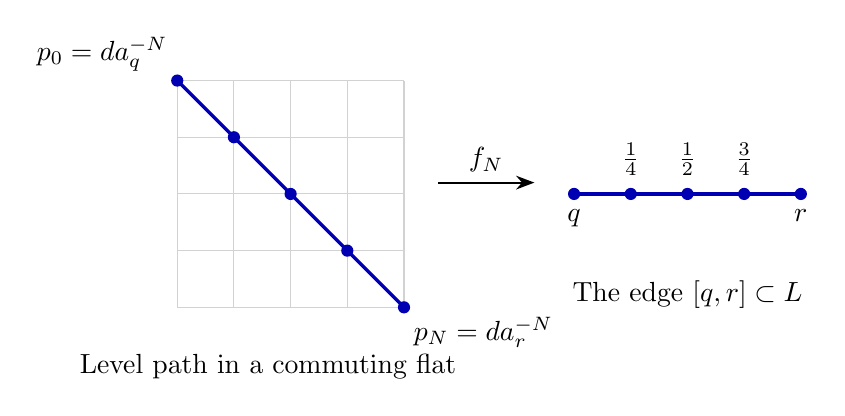
\begin{tikzpicture}[x=0.72cm,y=0.72cm,>=Stealth]
  \draw[step=1,gray!35,thin] (0,0) grid (4,4);
  \draw[blue!70!black,very thick] (0,4)--(4,0);
  \foreach \j in {0,...,4}{
   \fill[blue!70!black] (\j,{4-\j}) circle (2.2pt);
  }
  \node[above left] at (0,4) {$p_0=d a_q^{-N}$};
  \node[below right] at (4,0) {$p_N=d a_r^{-N}$};
  \node[below] at (1.6,-0.65) {Level path in a commuting flat};
  \draw[->,thick] (4.6,2.2)--node[above] {$f_N$}(6.3,2.2);
  \draw[blue!70!black,very thick] (7,2)--(11,2);
  \foreach \j in {0,...,4}{
   \fill[blue!70!black] ({7+\j},2) circle (2.2pt);
  }
  \node[below] at (7,1.9) {$q$};
  \node[below] at (11,1.9) {$r$};
  \node[above] at (8,2.15) {$\frac14$};
  \node[above] at (9,2.15) {$\frac12$};
  \node[above] at (10,2.15) {$\frac34$};
  \node[below] at (9,0.65) {The edge $[q,r]\subset L$};
 \end{tikzpicture}
 \caption{The special path~\eqref{eq:commuting-power-path}, shown for
 $N=4$, joins $d a_q^{-N}$ to $d a_r^{-N}$ across level-cut squares.
 Formula~\eqref{eq:exact-subdivision} sends it to the exact subdivision
 of $[q,r]$.  Here $a_q,a_r$ commute and $\lambda(d)=N$.
 Each blue diagonal step multiplies by $a_q a_r^{-1}$, preserving
 height zero; $f_N$ is shown on this level path.}
 \label{fig:commuting-path}
\end{figure}

We have obtained both properties needed from $f_N$: every triangle
boundary has small image, and selected closed paths trace prescribed
loops of $L$ exactly. The representation $\alpha$ will turn these two
properties into flatness on triangles and nontrivial closed-path
holonomy, respectively.

\subsection{Pulling back transport}

\begin{proof}[Proof of Proposition~\ref{prop:small-labels}]
Choose a base vertex $q_0$ for $\alpha$ and a base lift of $q_0$ in
the universal cover $\widetilde L\to L$.  Choose the left deck
action convention so that lifting a loop representing $\gamma$ from
that base lift ends at $\gamma$ times the lift.  There is a
continuous map
\begin{equation}\label{eq:developing-map}
 D:\widetilde L\longrightarrow H,
 \qquad D(\gamma\xi)=\alpha(\gamma)D(\xi).
\end{equation}
To construct it, choose images for representatives of the vertex
orbits and extend equivariantly.  On representatives of the edge
orbits, extend between the prescribed endpoints using path
connectedness of $H$.  Extend over representatives of the two-cell
orbits using $\pi_1(H)=0$.  The deck action is free on cells, so
equivariance introduces no ambiguity; $L$ has dimension two, so there
are no further extensions.  The CW topology gives continuity.

Fix $\epsilon>0$.  There is a finite open cover $(U_i)$ of $L$ such
that each $U_i$ is evenly covered and $D$ has image of diameter less
than $\epsilon$ on each sheet over $U_i$.  Indeed, around any lift
of a point, continuity of $D$ gives a sufficiently small such
neighborhood on one sheet.  All other sheets are its deck translates,
and left multiplication by $\alpha(\gamma)$ preserves quaternion
distance.  Compactness of $L$ then gives a finite subcover.  Let
$\ell>0$ be a Lebesgue number in the diameter form: every subset of
$L$ of diameter less than $\ell$ lies in some $U_i$.  Choose $N\geq2$
so large that $8/N<\ell$, and construct $f_N$ as above.

For an oriented edge $e$ of $X$, lift its assigned path $f_N(e)$ from
$\xi$ to $\xi'$ in $\widetilde L$, and define
\begin{equation}\label{eq:edge-transport}
 h_e=D(\xi)^{-1}D(\xi').
\end{equation}
Changing the lift multiplies both $D$ values on the left by the same
$\alpha(\gamma)$, so the label is independent of the lift.  Reversing
the path inverts the label.  Its image lies in some $U_i$ because its
diameter is at most $4/N<\ell$.  The lift stays in one sheet, and
therefore
\[
 |h_e-1|=|D(\xi')-D(\xi)|<\epsilon.
\]

The whole image of the boundary of a triangular two-cell lies in one
$U_i$ by~\eqref{eq:small-triangle-image}.  The inverse homeomorphism
of a sheet over $U_i$ lifts this boundary to a closed loop in that
sheet.  In multiplying the three edge
labels, choose these consecutive lifts; the intermediate $D$ values
cancel, giving product $1$.

Finally, choose a finite edge loop based at $q_0$,
$q_0,q_1,\ldots,q_k=q_0$ in $L$ whose class $\gamma$ has
$\alpha(\gamma)\ne1$.  Such a loop exists because $\alpha$ is
nontrivial and every element of the fundamental group of a simplicial
complex is represented by a finite edge loop.  For each successive
pair, concatenate the path~\eqref{eq:commuting-power-path}.  The
endpoint of each piece is $d a_{q_{i+1}}^{-N}$, the initial vertex of
the next piece, so this is a closed edge path in $X$ based at
$d a_{q_0}^{-N}$.  By~\eqref{eq:exact-subdivision}, its image under
$f_N$ is precisely the chosen loop with each edge subdivided.
Lift that image from the chosen base lift $\xi$ of $q_0$.  The terminal lift is
$\gamma\xi$, and telescoping~\eqref{eq:edge-transport} gives the
path product
\[
 D(\xi)^{-1}D(\gamma\xi)
 =D(\xi)^{-1}\alpha(\gamma)D(\xi)\ne1.
\]
This proves all assertions of the proposition.
\end{proof}

\subsection*{Completion of the proof of Theorem~\ref{thm:main}}
\addcontentsline{toc}{subsection}{Completion of the proof}

Choose the finite acyclic flag complex and the nontrivial representation from Section~\ref{sec:geometry}. Proposition~\ref{prop:model} gives a finitely generated residually finite group $G$ of integral cohomological dimension two, together with finite lists $S,\mathcal D$ satisfying the cycle-basis hypothesis of Theorem~\ref{thm:presentation}. If a two-dimensional classifying space for $G$ existed, that theorem would supply a positive threshold $\eta$. Proposition~\ref{prop:small-labels}, applied below this threshold, supplies labels with trivial product around every translate of every word in $\mathcal D$ but nontrivial product on a closed path. This is a contradiction.

The three-dimensional contractible complex $E$ of Section~\ref{sec:geometry} carries a free cellular action of $G$, so $E/G$ is a three-dimensional classifying space. Therefore $\gdim G=3$, whereas $\cdim G=2$. This completes the proof of Theorem~\ref{thm:main}.\qed

\bibliographystyle{plain}
\bibliography{references}
\end{document}
